\chapter{Raccolta dati ed implementazione}
\label{chap:implementazione}

Questo capitolo si occuperà, prima di tutto, di fornire dettagli sulle tecnologie e sulle modalità di raccolta dei dati da \textit{Twitter}, necessari alla costruzione di \textit{retweet graphs} associati ad \textit{hashtags} in \textit{input}.
\\Infine verrà trattata puntualmente l'implementazione degli algoritmi, definiti rigorosamente nel capitolo precedente, e di tutte quelle tecniche che hanno permesso di raggiungere l'obiettivo preposto, ovvero l'implementazione di un \textit{framework} che permetta di:
\begin{enumerate}
\item costruire ed analizzare \textit{retweet graphs} associati ad \textit{hashtags di Twitter} in \textit{input};
\item rilevare le \textit{echo-chambers} che caratterizzano la discussione;
\item eseguire un algoritmo di \textit{k-edge recommendation}, in modalità \textit{greedy} o meno;
\item fornire strumenti per l'analisi degli archi consigliati e per la visualizzazione dei nodi coinvolti (i.e. i nodi estremi degli archi consigliati).  
\end{enumerate}

\section{Raccolta dati}
La raccolta dei dati è una fase indispensabile, una condizione \textit{sine qua non}, senza la quale non è pensabile raggiungere alcun obiettivo tra quelli prefissati.
\\Poiché il \textit{software} proposto si occupa di \textit{endorsement graphs} del \textit{social network} di \textit{Twitter}, per la raccolta dei dati si è reso necessario l'utilizzo della \textit{Twitter Api}. Inoltre, visto che il linguaggio utilizzato per l'implementazione è \textit{Python}, sono state sfruttate le funzionalità della libreria \textit{Tweepy}, una via di accesso alla \textit{Twitter Api} di facile utilizzo. 
\\Nel seguito saranno forniti dettagli sugli strumenti di \textit{Twitter Api e Tweepy} e su altre tecniche che hanno permesso di \textit{bypassare} importanti limitazioni temporali delle \textit{Api di Twitter}.  

\subsection{Twitter Api}
\textit{Twitter} mette a disposizione degli sviluppatori delle \textit{Api}, utili per l'acquisizione dei dati pubblicati dagli utenti. Per rendere possibile il loro utilizzo bisogna innanzitutto creare un \textit{account Twitter} e poi effettuare l'iscrizione al \textit{reparto sviluppatori di Twitter}. Questa procedura è molto rigida e qualora non fosse seguita in modo rigoroso non sarebbe possibile utilizzare le \textit{Api}. 
\\Una volta effettuata l'iscrizione al \textit{reparto sviluppatori di Twitter}, è finalmente possibile procedere con la raccolta dei dati pubblicati dagli utenti, ma non prima di aver ottenuto le credenziali di accesso. Le credenziali vengono rilasciate a seguito della creazione di una \textit{Twitter App}, che rappresenta un \textit{progetto Twitter} dello sviluppatore: esse permetteranno di autenticarsi presso un \textit{server di Twitter}, con il quale sarà possibile interagire \textit{via streaming} mediante le \textit{Twitter Api} per ottenere i dati richiesti. Le credenziali si dividono in \textit{Token} e \textit{Consumer}, i quali hanno le seguenti caratteristiche e funzioni:
\begin{itemize}
\item il \textit{Token} permette l'accesso ai servizi che offre \textit{Twitter}. Non è sufficiente per consentire lo \textit{streaming} dei dati dal \textit{server}. \`E costituito da:
\begin{itemize}
\item \textit{Access Token};
\item \textit{Access Secret}.
\end{itemize}
\item il \textit{Consumer} consente lo \textit{streaming} dei dati di \textit{Twitter} dal \textit{server}. \`E costituito da:
\begin{itemize}
\item \textit{Consumer Key};
\item \textit{Consumer Secret}.
\end{itemize}
\end{itemize}
Nell'ambito della stessa \textit{Twitter App}, queste chiavi possono essere rigenerate a piacimento, anche con l'obiettivo di evitare problematiche relavite alla sicurezza. Qualunque sia il linguaggio di programmazione utilizzato per lo sviluppo del \textit{software} (nel caso in esame \textit{Python}), per utilizzare le \textit{Api} da codice è sempre necessario prima autenticarsi, fornendo tutti e quattro i codici appena elencati: le interfacce d'accesso alle \textit{Api} di \textit{Twitter} tuttavia dipendono dal linguaggio di programmazione e, nel nostro caso, sono realizzate mediante la libreria di \textit{Python Tweepy}, della quale parleremo nel seguito della trattazione.
\\Ad ogni modo, bisogna sottolineare che lo \textit{streaming} dei dati viene limitato da \textit{Twitter} per evitare che gli sviluppatori utilizzino in modo sconveniente i dati pubblicati dagli utenti: uno sviluppatore, pur essendo dotato di tutte le credenziali necessarie, non può effettuare più di 100 richieste ogni 15 minuti. Durante il tempo di pausa, che viene fatto scattare in corrispondenza del superamento della soglia di richieste, lo sviluppatore può decidere di aspettare che esso si esaurisca o, al contrario, può decidere deliberatamente di violarlo ed effettuare una nuova richiesta: in tal caso le sue credenziale verrebbero bloccate e non gli sarebbe permesso di comunicare con il \textit{server} mediante le \textit{Api} per circa un'ora.
\\Un'altra limitazione che impone l'\textit{Api} ufficiale di \textit{Twitter} riguarda l'impossibilità di ottenere \textit{tweets} più vecchi di una settimana: questa limitazione è molto forte ed ha costituito, nel processo di sviluppo del \textit{framework} proposto, un problema molto ingente, la cui risoluzione è dovuta alla libreria \textit{GetOldTweets di Python}, della quale parleremo presto.
\\Per terminare, i dati che lo sviluppatore richiede al \textit{server} mediante la \textit{Twitter Api} vengono restituiti in un file \textit{JSON}: esso conterrà tutti i \textit{metadati} necessari, i quali dipendono dal criterio della \textit{query}, come ad esempio il testo del \textit{tweet}, gli \textit{hashtags}, lo \textit{username} dell'utente che l'ha pubblicato e gli utenti che l'hanno \textit{retweettato}.

\subsection{Tweepy}
\textit{Tweepy} è una libreria di \textit{Python} che permette di accedere agevolmente alle \textit{Api} di \textit{Twitter}. Gestisce l'autenticazione dello sviluppatore presso il server di \textit{streaming} utilizzando i seguenti metodi:
\begin{enumerate}
\item \textit{tweepy.OAuthHandler(CONSUMER\_KEY, CONSUMER\_SECRET)}: 
\\una volta forniti \textit{Consumer Key e Consumer Secret} validi, restituisce un codice di autenticazione \textit{auth}; 
\item \textit{auth.set\_access\_token(ACCESS\_TOKEN, ACCESS\_TOKEN\_SECRET)}: 
\\permette di impostare il codice \textit{auth} con gli \textit{Access Token e Access Token Secret} (validi);
\item \textit{tweepy.API(auth)}: restituisce, in caso di corretta autenticazione, un oggetto \textit{Api} attraverso il quale può finalmente avvenire il processo di \textit{streaming} dal \textit{server}.
\end{enumerate}
Inoltre \textit{Tweepy} permette di gestire vari tipi di errore tra cui \textit{RateLimitError}, che insorge quando viene superata la soglia di traffico di 100 richieste ogni 15 minuti.

\subsection{GetOldTweets}
Come precedentemente detto, l'\textit{Api} ufficiale di \textit{Twitter} rende impossibile, con un semplice \textit{account} gratuito, l'acquisizione di \textit{tweets} più vecchi di una settimana. Questa limitazione, nel caso del sistema proposto, è intollerabile, visto che, per costruire \textit{retweet graphs} di dimensioni sufficienti a condurre un'analisi significativa, bisogna utilizzare un intervallo di osservazione abbastanza ampio. Superare tale limitazione continuando ad utilizzare l'\textit{Api} ufficiale vorrebbe dire pagare per ottenere un \textit{account Enterprise}, cosa che non siamo disposti a fare. 
\\La libreria \textit{GetOldTweets} permette di \textit{bypassare} l'\textit{Api} ufficiale e di ottenere \textit{tweets} più vecchi di una settimana semplicemente sfruttando la funzione \textit{scroll} della pagina di \textit{Twitter}: facendo \textit{scroll} verso il fondo pagina è possibile ottenere, tramite chiamate successive ad un \textit{provider JSON}, \textit{tweets} (relativi all'\textit{hashtag} che si sta cercando) via via più vecchi, evitando di incorrere a limitazioni temporali. Tale libreria mette a disposizione un gran numero di criteri di ricerca, utilizzati poi come parametri dell'indirizzo \textit{http}. Nel caso in esame sono stati utilizzati i seguenti parametri:
\begin{itemize}
\item \textit{Since}: una data limite inferiore per limitare la ricerca;
\item \textit{Until}: una data limite superiore per limitare la ricerca;
\item \textit{QuerySearch}: il testo di \textit{query} desiderato. Nel caso in esame, come \textit{query} viene sempre specificato un \textit{hashtag}, il quale identifica una discussione, e vengono considerati tutti e soli i \textit{tweets} creati nell'intervallo temporale specificato e che recano tale \textit{hashtag}.
\end{itemize}
Una volta costruito un oggetto \textit{tweetCriteria}, specificando le informazioni sopra elencate, esso viene passato come parametro al metodo \textit{getTweets} della classe \textit{TweetManager}, il quale si occupa di recuperare tutti i \textit{tweets} che soddisfano i criteri di ricerca. In particolare questo metodo, una volta costruita la \textit{url} contenente tutti i parametri di ricerca specificati, acquisisce la pagina \textit{web} contenente tutti i \textit{tweets} che soddisfano i criteri e converte il risultato in un formato \textit{JSON}. Le informazioni che, nel caso specifico dell'implementazione proposta, vengono estratte dai \textit{tweets} risultanti sono due:
\begin{itemize}
\item \textit{ID} del \textit{tweet};
\item \textit{Username} dell'autore del \textit{tweet}.
\end{itemize}
Gli \textit{ID} dei \textit{tweets} verranno utilizzati per recuperare tutti i \textit{retweets} associati, i quali sono indispensabili per costruire il \textit{retweet graph}.

\subsection{Processo di raccolta dati}
Descritte le caratteristiche e le peculiarità degli strumenti utilizzati per effettuare la raccolta dei dati, ora occorre analizzare il processo che permette di acquisirli e di renderli persistenti. Con tale obiettivo è stata implementata la classe \textit{TwittersRetweets}. Essa fornisce metodi per: 
\begin{enumerate}
\item Specificare i parametri di ricerca (i.e. \textit{Since,Until,QuerySearch}); 
\item Recuperare dal \textit{social network di Twitter} tutti i \textit{tweets} che soddisfano i parametri di ricerca specificati al punto \textit{1.}, insieme agli utenti che li hanno prodotti; 
\item Recuperare tutti i \textit{retweets} che sono stati prodotti verso i \textit{tweets} recuperati al punto \textit{2.};
\item Organizzare i dati ottenuti in un \textit{file} e renderli persistenti.
\end{enumerate}
Un oggetto della classe \textit{TwittersRetweets} ha pertanto i seguenti attributi:
\begin{itemize}
\item \textit{since}, ossia la data di inizio ricerca; 
\item \textit{until}, ossia la data di fine ricerca;
\item \textit{query}, utilizzato, nel caso in esame, per specificare un \textit{hashtag};
\item \textit{twittapi}, ossia l'oggetto \textit{api}, senza il quale è impossibile eseguire lo \textit{streaming}, ottenuto a seguito dell'autenticazione presso un \textit{server} di \textit{Twitter} mediante l'utilizzo della libreria \textit{Tweepy}.
\end{itemize}
Il processo di raccolta dati viene eseguito mediante l'invocazione del metodo \textit{computeRetweets(path)} su un oggetto della classe \textit{TwittersRetweets} che ha come attributi proprio i parametri di ricerca (i.e. \textit{since, until, query}) e l'oggetto \textit{twittapi}.
L'esecuzione del metodo \textit{computeRetweets(path)} si articola in tre fasi, come è possibile evincere dalla figura \ref{fig:raccolta_dati}. Più precisamente:
\begin{enumerate}
\item Il metodo \textit{computeRetweets(path)} innanzittutto si occupa di recuperare tutti i \textit{tweets} che soddisfano i parametri di ricerca e gli utenti che li hanno creati. Per fare questo, viste le limitazioni temporali che impone l'\textit{Api} ufficiale di \textit{Twitter}, si rende necessario l'utilizzo della libreria \textit{GetOldTweets}: vengono specificati i criteri di ricerca dei \textit{tweets} da recuperare ed infine il \textit{TweetManager} si occupa di cercarli nella pagina \textit{html} di \textit{Twitter}, per poi restituirli. I \textit{tweets} restituiti sono caratterizzati da due importanti parametri: \textit{tweetid}, ossia l'identificativo univoco del \textit{tweet}, e lo \textit{username}, ossia l'utente che l'ha emesso. Per mezzo di questi parametri, in questa fase vengono costruiti due oggetti, ossia:
\begin{itemize}
\item \textit{dictioTwitters}: un dizionario che ha come chiavi gli \textit{usernames} degli utenti che hanno emesso i \textit{tweets} recuperati e come valori dei dizionari della forma \textit{\{'tweetcount' : x\}}, dove \textit{x} è il numero dei \textit{tweets} recuperati (e che quindi soddisfano i criteri di ricerca) che sono attribuibili ad un certo \textit{username};
\item \textit{tweetids}: una lista che ha come elementi dei dizionari della forma \textit{\{tweetid : tweetuser\}}, dove \textit{tweetid} identifica un certo \textit{tweet} e \textit{tweetuser} identifica l'utente che l'ha emesso.
\end{itemize}
Questi oggetti vengono opportunamente popolati e poi forniti come \textit{input} alla fase successiva.
\item La fase \textit{2} si occupa di scansionare la lista \textit{tweetids}, restituita dalla fase precedente, per individuare tutti i \textit{retweets} emessi nei confronti dei \textit{tweets} che soddisfano i criteri di ricerca. A fine scansione, questa fase restituisce il dizionario \textit{dictioRetweets}, che ha come chiavi delle tuple del tipo \textit{(retweetuser,tweetuser)}, dove \textit{retweetuser} è lo \textit{username} di un utente che ha \textit{retweettato} almeno un \textit{tweet} emesso dall'utente identificato da \textit{tweetuser}, e come valori dei dizionari del tipo \textit{\{'retweetcount' : x\}}, dove \textit{x} è il numero di volte che l'utente \textit{retweetuser} ha \textit{retweettato} dei contenuti dell'utente \textit{tweetuser}. 
\\Questa volta, tuttavia, tali \textit{retweets} sono ottenuti per mezzo dell'\textit{Api} ufficiale di \textit{Twitter}. In particolare, per ogni elemento \textit{\{tweetid : tweetuser\}} della lista \textit{tweetids}:
\begin{enumerate}
\item mediante l'invocazione del metodo \textit{retweets}, messo a disposizione dalla \textit{Twitter Api}, vengono recuperati tutti i \textit{retweets} emessi nei confronti del \textit{tweet} identificato dal \textit{tweetid}. Tali \textit{retweets} vengono restituiti sotto forma di una lista di \textit{status objects}, un formato particolare che viene gestito dalla \textit{Twitter Api};
\item per ogni \textit{status object}, che corrisponde ad un particolare \textit{retweet}, viene recuperato il \textit{JSON} che lo descrive, da cui viene estratto lo \textit{username} dell'utente che ha effettuato il \textit{retweet} stesso (accedendo opportunamente ai campi del \textit{JSON}), che chiamiamo \textit{retweetuser}. Se la tupla \textit{(retweetuser,tweetuser)} esiste già come chiave nel dizionario \textit{dictioRetweets} allora viene semplicemente aggiornato il valore del campo \textit{'retweetcount'} corrispondente, altrimenti tale tupla viene aggiunta al dizionario come sua nuova chiave con valore \textit{\{'retweetcount' : 1\}}. 
\\Infine, se lo \textit{username} \textit{retweetuser} non è presente come chiave nel dizionario \textit{dictioTwitters}, viene aggiunta la nuova chiave \textit{retweetuser} con valore \textit{\{'tweetcount' : 0\}}, in quanto \textit{retweetuser} non ha mai emesso \textit{tweets} contenenti l'\textit{hashtag} specificato.
\end{enumerate}
Il blocco di codice che implementa le azioni descritte nei precedenti punti (a) e (b) è opportunamente gestito da una clausola \textit{try}: in effetti, come precedentemente detto, l'invocazione del metodo \textit{retweets} della \textit{Twitter Api}, in caso di superamento della soglia di 100 richieste ogni 15 minuti, potrebbe causare il sollevamento dell'eccezione \textit{tweepy.error.RateLimitError}. Tale eccezione verrebbe gestita nella clausola \textit{except} immediatamente successiva, mettendo in pausa il processo di acquisizione dei \textit{retweets} per 15 minuti, in modo tale da non incorrere al blocco di un'ora delle credenziali;
\item Acquisite le informazioni necessarie alla costruzione del \textit{retweet graph} corrispondente alla \textit{query} (ossia all'\textit{hashtag}) ed all'intervallo temporale \textit{since-until} forniti in input, è possibile procedere con il loro salvataggio in memoria. Infatti, giunto a questa fase, il metodo \textit{computeRetweets(path)} si occupa di rendere persistenti i dati collezionati nel dizionario \textit{dictioRetweets}. Innanzitutto apre il file di testo corrispondente al \textit{path} fornito in input e successivamente, per ogni chiave \textit{key} in \textit{dictioRetweets}, si occupa di salvarvi le informazioni nel formato \textit{"key[0],key[1],retweetcount"}, andando a capo per ogni \textit{entry} inserita. Ricordiamo che \textit{key[0]} è \textit{retweetuser}, \textit{key[1]} è \textit{tweetuser} e \textit{retweetcount} è il numero di volte che \textit{retweetuser} ha \textit{retweettato} \textit{tweets} di \textit{tweetuser}.
\\In figura \ref{fig:retweet_file} è possibile osservare un esempio di tale file di testo.
\\Bisogna sottolineare che questo formato di salvataggio dei dati è stato scelto anche per motivi di compatibilità con lo schema utilizzato dall'articolo \cite{garimella:paper}, in modo tale da poterne riprodurre facilmente i test.
\\\\
\end{enumerate}

\begin{figure}
\begin{center}
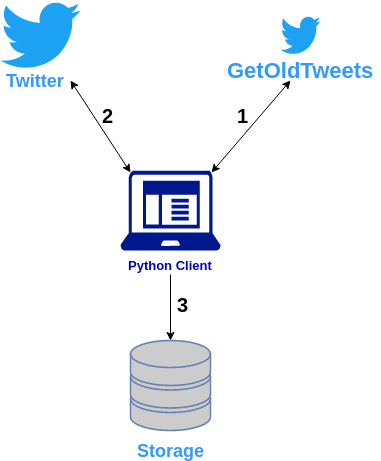
\includegraphics[scale=0.6]{images/raccolta_dati_tesi.png}
\end{center}
\caption{Processo di raccolta dati.}
\label{fig:raccolta_dati}
\end{figure}

\begin{figure}
\begin{center}
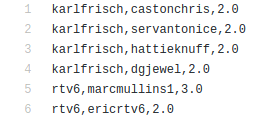
\includegraphics[scale=0.6]{images/retweet_input_file.png}
\end{center}
\caption{Esempio di file che descrive un \textit{retweet graph}.}
\label{fig:retweet_file}
\end{figure}

\section{Implementazione}
In questo paragrafo verrà descritta l'implementazione di tutte quelle fasi che sono successive alla raccolta dati. Fissato un certo \textit{hashtag} che identifica una discussione che ha luogo su \textit{Twitter} ed un intervallo di osservazione, i dati vengono raccolti come illustrato nel paragrafo precedente, per poi essere convertiti in un vero e proprio \textit{retweet graph}, per il quale è possibile:
\begin{enumerate}
\item rilevere le \textit{echo-chambers} e calcolare l'\textit{RWC};
\item eseguire i due algoritmi di \textit{k-edge recommendation}.
\end{enumerate}
In figura \ref{fig:pipe} è sintetizzato tutto il processo al quale viene sottoposto il grafo, che infine conduce ai risultati derivanti dall'applicazione dei due algoritmi alternativi proposti.

\begin{figure}
\begin{center}
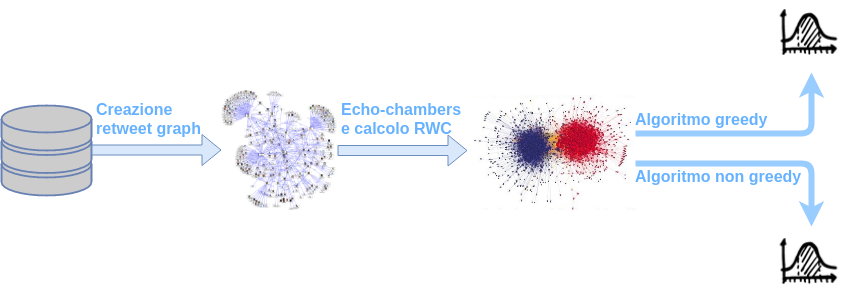
\includegraphics[scale=0.56]{images/pipeline_implementazione.png}
\end{center}
\caption{\textit{Pipeline} implementativa.}
\label{fig:pipe}
\end{figure}
Nel seguito della trattazione verranno illustrati tutti i dettagli implementativi delle fasi di cui si compone la \textit{pipeline} in figura, iniziando dalla fase di creazione del \textit{retweet graph}.

\subsection{Creazione del \textit{retweet graph}}
Per eseguire agevolmente tutte le operazioni di manipolazione ed analisi dei grafi utili al raggiungimento degli obiettivi sopra menzionati, è necessario rappresentare i \textit{retweet graphs} con un formato facilmente gestibile dal linguaggio \textit{Python}. La fase di raccolta dati, illustrata nel paragrafo precedente, al termine della sua esecuzione si preoccupa di rendere persistenti le informazioni raccolte. Tali informazioni sono certamente sufficienti a descrivere il \textit{retweet graph} a cui si riferiscono ma sono caratterizzate da un formato non facilmente manipolabile via codice: occorre rappresentare tali informazioni mediante una struttura dati.
\\A tale scopo, la classe \textit{EndorsementGraph}, che ha come attributi il \textit{path} del file di testo in input ed il suo nome, permette di:
\begin{enumerate}
\item \textit{parsare} il contenuto del file di testo in input, creato nella fase di raccolta dati, per ottenere una struttura dati che rappresenti il \textit{retweet graph} corrispondente;
\item \textit{serializzare} la struttura dati creata e rendere persistente il risultato della serializzazione.
\end{enumerate}
In sintesi, la classe \textit{EndorsementGraph} permette di modellare un \textit{retweet graph}, corrispondente a determinati criteri di ricerca \textit{(querySearch,since,until)} e le cui informazioni sono state già raccolte ed organizzate in un file, con una struttura dati direttamente manipolabile da codice. 
Il \textit{core} della classe \textit{EndorsementGraph} è il metodo \textit{buildEGraph}, il quale si occupa di costruire tale struttura dati e di serializzarla, per poi memorizzare il risultato della serializzazione nella \textit{directory} il cui \textit{path} è specificato come parametro.
\\Il metodo \textit{buildEGraph} demanda al \textit{package NetworkX} la creazione della struttura dati che descrive il \textit{retweet graph} considerato e la sua manipolazione. In particolare, \textit{NetworkX} è un pacchetto \textit{Python} per la creazione, la manipolazione e lo studio della struttura, delle dinamiche e delle funzioni di reti complesse. Tra le altre \textit{features}, in particolare offre strumenti per lo studio della struttura e della dinamica delle reti sociali, biologiche e infrastrutturali, strumenti che sono stati largamente sfruttati nel lavoro di tesi proposto.
\\Scendiamo ora nei dettagli implementativi del metodo \textit{buildEGraph(destination\_dir)}. Esso viene invocato su un oggetto della classe \textit{EndorsementGraph}, caratterizzato dagli attributi \textit{input\_dir} e \textit{input\_name}, ossia, rispettivamente, la \textit{directory} e il nome del file di testo che descrive il \textit{retweet graph} in considerazione, file creato nella fase di raccolta dati.
\\Il metodo \textit{buildEGraph} costruisce un \textit{DiGraph} (i.e. grafo diretto) di \textit{NetworkX} a partire dalle informazioni collezionate nel file \textit{input\_name} attraverso i seguenti passi:
\begin{enumerate}
\item Crea tre dizionari:
\begin{itemize}
\item \textit{dictio\_nodes\_convert}, in cui ogni chiave è l'\textit{username} di un utente che ha partecipato alla discussione ed il valore corrispondente è un suo identificativo univoco; 
\item \textit{dictio\_nodes}, in cui ogni chiave è l'\textit{username} di un utente che ha partecipato alla discussione ed il valore corrispondente è il numero di volte che tale utente ha effettuato un \textit{retweet} sul \textit{topic} in questione;
\item \textit{dictio\_edges}, in cui ogni chiave identifica una relazione di \textit{endorsement} \textit{(source,dest)}, dove \textit{source e dest} sono due \textit{usernames}, ed il valore corrispondente è il numero di volte che l'utente \textit{source} ha effettuato un \textit{retweet} nei confronti dell'utente \textit{dest}.
\end{itemize}
\item Popola tali dizionari \textit{parsando} il file \textit{input\_name}, riga per riga, dove ogni riga ha la forma \textit{"source,dest,retweetcount"}, in modo tale che, al termine del \textit{parsing}:
\begin{itemize}
\item sia possibile associare ad ogni \textit{username} di utenti che hanno partecipato alla discussione un identificativo, ossia \textit{dictio\_nodes\_convert[username]};
\item sia possibile associare ad ogni arco \textit{(source,dest)} una tupla di identificativi \textit{(dictio\_nodes\_convert[source],dictio\_nodes\_convert[dest])};
\item sia possibile associare ad ogni tupla \textit{(dictio\_nodes\_convert[source],\\dictio\_nodes\_convert[dest])} una probabilità di \textit{retweet} pari a:  

\begin{equation}
P[(source,dest)] = \frac{dictio\_edges[(source,dest)]}{dictio\_nodes[source]}
\end{equation}

\end{itemize}
\item Utilizzando le informazioni ottenute al passo precedente, il metodo \textit{buildEGraph} popola il \textit{DiGraph} con dei nodi, identificati da un intero univoco e che hanno come attributi il proprio \textit{retweetcount} (i.e. il numero di volte che l'utente corrispondente al nodo ha effettuato un \textit{retweet} sul \textit{topic} in questione) ed il proprio \textit{username}, e degli archi diretti, che hanno come unico attributo una probabilità di \textit{retweet}, ricavata dalla formula (3.1);

\item Serializza il \textit{DiGraph} ottenuto mediante l'utilizzo del modulo \textit{Pickle}, il quale implementa i protocolli binari per la serializzazione e la de-serializzazione di una struttura di oggetti Python. Infine si preoccupa di rendere persistente il risultato della serializzazione: ciò consente di riutilizzare in futuro il \textit{retweet graph} creato, evitando di dover rieseguire il \textit{parsing}, semplicemente invocando l'operazione di \textit{unpickling} sulla versione serializzata, ottenendo nuovamente l'oggetto originario.  
\end{enumerate}
Bisogna sottolineare il fatto che la probabilità di \textit{retweet} (3.1), seppur presente come attributo degli archi del \textit{DiGraph}, non è stata utilizzata nell'implementazione proposta ma è stata comunque inserita per permettere futuri sviluppi del \textit{framework}.
\\
\subsection{Individuazione delle \textit{echo-chambers}}

Il metodo \textit{computeData} del modulo \textit{utilities} si occupa di individuare le \textit{echo-chambers} del \textit{retweet graph} in input, le quali sono indispensabili per ricavare tutti i componenti necessari al calcolo del \textit{random-walk controversy score} ed all'esecuzione degli algoritmi di \textit{k-edge recommendation}.
\\Come detto nel capitolo precedente, le \textit{echo-chambers} vengono individuate mediante l'esecuzione dell'algoritmo di \textit{Girvan-Newman}, la cui implementazione è resa disponibile dal \textit{package NetworkX}. Tale implementazione richiede di convertire il grafo in input nella sua versione \textit{non diretta} (i.e. grafo \textit{non orientato}), ma nulla vieta in futuro di estendere il codice in modo tale che riesca a gestire anche grafi diretti. 
Il risultato dell'esecuzione dell'algoritmo di \textit{Girvan-Newman} viene gestito dal metodo \textit{computeData} con l'ausilio dei seguenti dizionari:
\begin{itemize}
\item \textit{communities}, in cui ogni chiave corrisponde all'indice di una delle comunità rilevate dall'algoritmo ed il valore corrispondente altro non è che la lista dei nodi del grafo che appartengono a tale comunità; 
\item \textit{partitions}, in cui ogni chiave è un nodo del grafo ed il valore corrispondente è l'indice della comunità a cui tale nodo appartiene.
\end{itemize}
I dizionari \textit{communities e partitions} permettono di partizionare perfettamente l'insieme dei nodi del grafo, in modo tale che ciascuno di essi venga associato all'\textit{echo-chamber} a cui appartiene, ossia al lato della \textit{controversia} per il quale si schiera. Nei paragrafi a seguire, sarà possibile notare quanto tali dizionari siano largamente usati ed indispensabili per l'esecuzione del sistema proposto.
\\\`E necessario precisare che la scelta dell'algoritmo di \textit{Girvan-Newman} non è stata immediata ma, al contrario, precedentemente è stato valutato un algoritmo di \textit{community detection} alternativo, ossia l'algoritmo di \textit{Louvain}.  
\\Al contrario dell'algoritmo di \textit{Girvan-Newman}, il metodo di \textit{Louvain} non agisce rimuovendo ad ogni passo l'arco caratterizzato dall'\textit{edge betweenness} più alta ma è incentrato sull'ottimizzazione della \textit{modularità}, che misura la densità dei collegamenti all'interno delle comunità rispetto ai collegamenti tra le comunità. L'algoritmo inizia assegnando ciascun nodo alla propria comunità e consiste in due fasi:
\begin{enumerate}
\item \textit{modularity optimization}: in questa fase, per ciascun nodo l'algoritmo esamina quanto cambierebbe la modularità se il nodo venisse rimosso dalla sua comunità e aggiunto alla comunità di ciascuno dei suoi vicini. Il nodo viene quindi inserito nella comunità in cui viene massimizzato il guadagno in modularità. Questo processo viene ripetuto per ciascuno dei nodi fino a quando non è possibile ottenere ulteriori miglioramenti;
\item \textit{community aggregation}: l'algoritmo ora crea una nuova rete i cui nodi sono le comunità trovate nella prima fase.
\end{enumerate}
Queste fasi vengono ripetute in modo iterativo fino al raggiungimento della modularità massima. In sintesi, è possibile dire che l'approccio di \textit{Louvain} si basa su un processo di \textit{aggregazione} della rete mentre l'approccio di \textit{Girvan-Newman} si basa su un processo di \textit{decomposizione} della rete. 
\\Tuttavia il processo di \textit{aggregazione} di \textit{Louvain} è volto all'ottimizzazione della \textit{modularità} e quindi nel momento in cui si arresta potrebbe aver rilevato un numero di comunità maggiore di due; al contrario \textit{Girvan-Newman}, essendo caratterizzato da un processo di \textit{decomposizione}, può essere arrestato nel momento in cui rileva esattamente due comunità. 
\\Questo è sostanzialmente il motivo che ha condotto alla scelta dell'algoritmo di \textit{Girvan-Newman}, non tralasciando le motivazioni addotte nel precedente capitolo \textit{Teoria alla base del problema ed algoritmi per la risoluzione}.

\subsection{Calcolo dell'\textit{RWC}}
Una volta rilevate le \textit{echo-chambers} del \textit{retweet graph} in input, ossia il \textit{DiGraph} ricavato nella precedente fase di \textit{"creazione del retweet graph"}, è possibile ottenere tutte le componenti utili al calcolo dell'\textit{indice di controversia RWC}, le quali dipendono proprio dalla struttura delle comunità. 
\\Il processo di calcolo dell'\textit{RWC} del grafo in input è illustrato in figura \ref{fig:rwc}. 

\begin{figure}
\begin{center}
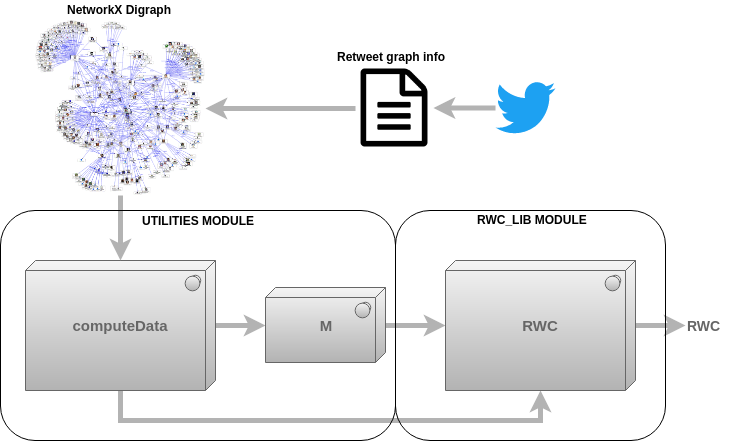
\includegraphics[scale=0.55]{images/calcolo_rwc.png}
\end{center}
\caption{Processo di calcolo del \textit{random-walk controversy score} di un \textit{retweet graph}.}
\label{fig:rwc}
\end{figure}
Come illustrato in figura, il \textit{DiGraph di NetworkX} ottenuto nella fase di \textit{"creazione del retweet graph"} viene fornito come input al metodo \textit{computeData} il quale, dopo averne individuato le \textit{echo-chambers}, produce\footnote{Oltre ai dati elencati, il metodo \textit{computeData} produce anche i dizionari \textit{communities,partitions} e le liste dei nodi delle due comunità \textit{sorted\_x,sorted\_y}, ordinate secondo l'\textit{in degree} dei nodi stessi. Ad ogni modo questi dati non sono utili al calcolo dell'\textit{RWC} e pertanto per il momento non verranno considerati.}:
\begin{itemize}
\item i vettori di \textit{restart} $e_x$ ed $e_y$, dove \textit{X,Y} indicano le due \textit{echo-chambers} del \textit{DiGraph}; 
\item i vettori $c_x$ e $c_y$;  
\item le matrici di transizione $P_x$ e $P_y$ e quindi le matrici $M_x\textsuperscript{-1}$ ed $M_y\textsuperscript{-1}$. 
\end{itemize}
Per chiarimenti riguardo il significato di questi vettori e matrici si consiglia la lettura del capitolo precedente.
\\Il metodo \textit{rwc} del modulo \textit{rwc\_lib} ha il compito di utilizzare questi dati per calcolare finalmente il \textit{random-walk controversy score} del \textit{DiGraph} in input, applicando la seguente espressione:
\\
\begin{equation}
RWC(G,X,Y) = (1 - \alpha)(c_x - c_y)\textsuperscript{T}(M_x\textsuperscript{-1}e_x - M_y\textsuperscript{-1}e_y)
\end{equation}
\\
Dove $\alpha$, fornito come parametro al metodo \textit{rwc}, è la \textit{probabilità di continuare il random-walk} e quindi $(1-\alpha)$ è la \textit{restart probability}. 
\\Come già precedentemente affermato, i due algoritmi alternativi di \textit{k-edge recommendation} sono stati implementati perseguendo anche l'obiettivo di limitare l'invocazione del metodo \textit{computeData}, poiché esso presenta un peso computazionale piuttosto ingente dovuto, tra le altre cose, al calcolo delle matrici inverse  $M_x\textsuperscript{-1}$ ed $M_y\textsuperscript{-1}$. 
\\L'esecuzione di entrambi gli algoritmi di \textit{k-edge recommendation} proposti richiede di calcolare, per ogni arco scansionato, il \textit{$\delta RWC$} che esso apporterebbe se fosse aggiunto al grafo. Se non si utilizzasse una strategia di calcolo più efficiente, per ottenere tale \textit{$\delta RWC$} bisognerebbe misurare l'\textit{RWC} del grafo a seguito dell'aggiunta dell'arco in considerazione, per poi effettuare la differenza con l'\textit{RWC} prima dell'aggiunta. Ciò renderebbe necessaria l'invocazione del metodo \textit{computeData} per un numero di volte pari al numero di archi scansionati, con l'effetto di un degrado prestazionale non trascurabile. \\Con l'obiettivo di ovviare a tutto ciò, l'implementazione proposta di entrambi gli algoritmi di \textit{k-edge recommendation} utilizza la tecnica di \textit{Sherman-Morrison}, già illustrata nel capitolo precedente, la quale permette di evitare di invocare continuamente il metodo \textit{computeData} per il calcolo dei \textit{$\delta RWC$}. 

\subsection{Implementazione degli algoritmi proposti}
Entrambi gli algoritmi di \textit{k-edge recommendation} implementati, ossia \textit{non greedy} e \textit{greedy}, scelgono i \textit{k} archi più promettenti, in termini del decremento dell'\textit{RWC} che consentirebbero se fossero aggiunti al grafo, partendo dallo stesso dominio. Tale dominio è costituito da tutti gli archi diretti, non ancora materializzati nel \textit{retweet graph} considerato, che connettono i \textit{$k_1$} vertici con \textit{in degree} più alto dell'\textit{echo-chamber X} con i \textit{$k_2$} vertici con \textit{in degree} più alto dell'\textit{echo-chamber Y} e viceversa, dove \textit{$k_1$} e \textit{$k_2$} devono essere forniti come input. 
\\I due algoritmi, come precedentemente affermato, differiscono tra loro solo per la modalità di selezione dei \textit{k} archi: questa differenza è facilmente deducibile dallo \textit{pseudo-codice} dei metodi che li implementano.

\begin{algorithm}
\caption{\textit{non\_greedy\_alg(g, data, X, Y, $\alpha$, $k_1$, $k_2$, k)}}
\begin{algorithmic} 
\STATE sorted\_x $\leftarrow$ sort\_nodes(g, X); 
\STATE sorted\_y $\leftarrow$ sort\_nodes(g, Y);
\STATE domain\_edges $\leftarrow$ get\_domain\_edges(g, $\alpha$, $k_1$, $k_2$, sorted\_x, sorted\_y, data);
\STATE sorted\_edges $\leftarrow$ sort\_by\_delta\_rwc(domain\_edges);
\STATE best\_edges $\leftarrow$ sorted\_edges[0:k];
\RETURN best\_edges;
\end{algorithmic}
\end{algorithm}

Osservando \textit{Algorithm 2 e Algorithm 3}, risulta subito evidente la minore complessità dello \textit{pseudo-codice} dell'algoritmo \textit{non-greedy} che, vedremo nei test, corrisponde ad una maggiore efficienza per quanto concerne i tempi di esecuzione ma anche ad una minore efficacia per quanto concerne il decremento dell'\textit{RWC}, rispetto a ciò che invece consente l'algoritmo \textit{greedy}.
\\Poniamo ora l'attenzione sullo \textit{pseudo-codice} dell'algoritmo \textit{non-greedy} e cerchiamo di analizzarlo, iniziando dai parametri in input:
\begin{itemize}
\item \textit{g} è il \textit{DiGraph} in input, ossia il \textit{retweet graph} (caratterizzato da un certo \textit{hashtag}) di cui si vuole ridurre il \textit{random-walk controversy score}; 
\item \textit{data} è l'insieme di vettori e matrici restituiti dal metodo \textit{computeData}, come osservato precedentemente;
\item \textit{X,Y} sono le due comunità (i.e. \textit{echo-chambers}) del grafo, anch'esse restituite dal metodo \textit{computeData} ed individuate mediante l'esecuzione dell'algoritmo di \textit{Girvan-Newman};
\item $\alpha$, $k_1$, $k_2$ e $k$ sono, rispettivamente, la \textit{probabilità di continuare il random-walk}, il numero di vertici con \textit{in degree} più alto della comunità \textit{X} da considerare, il numero di vertici con \textit{in degree} più alto della comunità \textit{Y} da considerare ed il numero di archi da consigliare. 
\end{itemize}
Come è possibile osservare dal suo \textit{pseudo-codice}, la modalità di selezione dei \textit{k} archi utilizzata dall'algoritmo \textit{non-greedy} si compone dei seguenti passi:
\begin{enumerate}
\item \textit{sorting} dei nodi della comunità \textit{X} e \textit{sorting} dei nodi della comunità \textit{Y} rispetto al loro \textit{in degree};
\item costruzione del dominio dei \textit{$2 \times k_1 \times k_2$} archi diretti che collegano i \textit{$k_1$} vertici con \textit{in degree} più alto dell'\textit{echo-chamber X} con i \textit{$k_2$} vertici con \textit{in degree} più alto dell'\textit{echo-chamber Y} e viceversa, tra i quali verranno scelti i \textit{k} più promettenti per la riduzione dell'\textit{RWC}. Bisogna sottolineare che tale dominio potrebbe contenere meno di  \textit{$2 \times k_1 \times k_2$} archi, qualora qualcuno di essi fosse già presente nel grafo. Nello \textit{pseudo-codice} questo passo viene espletato da \textit{get\_domain\_edges}, alla cui implementazione è richiesto anche di associare ad ogni arco del dominio il proprio \textit{$\delta RWC$}, calcolato mediante la tecnica di \textit{Sherman-Morrison};
\item \textit{sorting} degli archi del dominio individuato al punto precedente in ordine decrescente dei loro \textit{$\delta RWC$}, cambiati di segno. Nello \textit{pseudo-codice} questo passo viene espletato da \textit{sort\_by\_delta\_rwc};
\item \textit{return} dei \textit{top-k} archi dell'insieme ordinato al punto precedente, ossia i \textit{best\_edges}.
\end{enumerate}

\begin{algorithm}
\caption{\textit{greedy\_alg(g, data, X, Y, $\alpha$, $k_1$, $k_2$, k)}}
\begin{algorithmic} 
\STATE Initialization : best\_edges $\leftarrow$ [];
\FOR{\textit{i = 0:k}}
\STATE sorted\_x $\leftarrow$ sort\_nodes(g, X); 
\STATE sorted\_y $\leftarrow$ sort\_nodes(g, Y);
\STATE domain\_edges $\leftarrow$ get\_domain\_edges(g, $\alpha$, $k_1$, $k_2$, sorted\_x, sorted\_y, data);
\STATE sorted\_edges $\leftarrow$ sort\_by\_delta\_rwc(domain\_edges);
\STATE g.add\_edge(sorted\_edges[0]);
\STATE data $\leftarrow$ compute\_data(g, $\alpha$, X, Y);
\STATE best\_edges.append(sorted\_edges[0]);
\ENDFOR
\RETURN best\_edges;
\end{algorithmic}
\end{algorithm}

La versione \textit{greedy} dell'algoritmo di \textit{k-edge recommendation} è caratterizzata dagli stessi parametri in input della versione \textit{non-greedy} ma, come si osserva dal suo \textit{pseudo-codice}, differisce da quest'ultima per quanto riguarda la modalità di scelta dei \textit{k} archi da proporre. In particolare, si nota che in ognuno dei \textit{k} passi impiegati per individuare i \textit{k} archi esegue le seguenti operazioni:
\begin{enumerate}
\item \textit{sorting} dei nodi della comunità \textit{X} e \textit{sorting} dei nodi della comunità \textit{Y} rispetto al loro \textit{in degree};
\item costruzione del dominio dei \textit{$2 \times k_1 \times k_2$} archi diretti, come descritto al punto 2 dell'algoritmo \textit{non-greedy}; 
\item \textit{sorting} degli archi del dominio individuato al punto precedente, come descritto al punto 3 dell'algoritmo \textit{non-greedy};
\item aggiunta al grafo \textit{g} dell'arco diretto migliore, individuato al punto precedente. Per migliore si intende in termini del \textit{$\delta RWC$} associato. Nello \textit{pseudo-codice} questo passo viene espletato da \textit{add\_edge};
\item ricalcolo dell'oggetto \textit{data}, mediante l'invocazione del metodo \textit{computeData}, necessario a seguito dell'aggiunta del nuovo arco al grafo \textit{g}. Come è possibile notare dallo \textit{pseudo-codice}, in questo caso al metodo \textit{computeData} vengono passate come parametri anche le due \textit{echo-chambers X,Y}. L'algoritmo \textit{greedy}, infatti, assume che le due comunità \textit{X,Y} restino invariate a seguito delle aggiunte degli archi al grafo: per permettere questo, l'implementazione di \textit{computeData} consente di scegliere se specificare o meno le \textit{echo-chambers} come parametri in input e, in caso vengano specificate, esse non vengono ricalcolate nuovamente.
\\Oltretutto, l'esigenza dell'algoritmo \textit{greedy} di fissare le \textit{echo-chambers} consente di ottenere un vantaggio prestazionale, visto che permette di non eseguire continuamente l'algoritmo di \textit{Girvan-Newman}\footnote{In caso contrario, sarebbe stato necessario invocare l'algoritmo di \textit{Girvan-Newman} un numero di volte pari a \textit{k}, con l'effetto di un degrado prestazionale inaccettabile.}, il quale risulta oneroso soprattutto per grafi con molti nodi ed archi, come nel caso in esame;
\item aggiornamento della lista \textit{best\_edges} mediante l'aggiunta dell'arco diretto individuato al punto 3 (i.e. \textit{sorted\_edges[0]}).
\end{enumerate}
Al termine del \textit{loop}, l'algoritmo \textit{greedy} restituisce la lista dei \textit{k} archi costruita in \textit{k} passi, ovvero la lista \textit{best\_edges}.
\\Come già osservato precedentemente, l'algoritmo \textit{greedy} è senz'altro più lento dell'algoritmo \textit{non-greedy} di un fattore \textit{k}, visto che impiega \textit{k} passi per scegliere \textit{k} archi. Questa caratteristica, tuttavia, fa sì che la modalità di selezione degli archi adottata dalla versione \textit{greedy} sia più precisa e permetta, a parità di archi aggiunti, un maggiore decremento del \textit{random-walk controversy score} del grafo rispetto a quanto permette la versione \textit{non-greedy}. Il capitolo relativo ai test dimostrerà l'attendibilità di queste osservazioni.

\subsection{Strumento per la visualizzazione degli archi consigliati}
Sarebbe interessante confrontare i due algoritmi di \textit{k-edge recommendation} non solo dal punto di vista del decremento dell'\textit{RWC} che, a parità di archi proposti, consentono ma anche dal punto di vista delle caratteristiche dei nodi estremi (i.e. \textit{endpoints}) dei \textit{k} archi che scelgono. Infatti, poiché i due algoritmi differiscono per la modalità di scelta dei \textit{k} archi, anche i nodi (ossia gli utenti del \textit{social network}) che essi coinvolgono saranno, in generale, diversi. 
\\Pertanto la visualizzazione di tali nodi, e di alcune loro caratteristiche tra cui l'\textit{in-degree}, l'\textit{out-degree} e l'\textit{username} dell'utente al quale corrispondono, potrebbe essere uno strumento ausiliario per individuare le cause che fanno sì che un algoritmo sia più efficace dell'altro.
\\A tale scopo, il sistema proposto implementa un \textit{tool} di visualizzazione dei \textit{k} archi scelti e dei loro nodi estremi, descritti dal corrispondente \textit{username} e dal loro \textit{in} e \textit{out-degree}. In particolare, il \textit{tool} ha l'obiettivo di evidenziare i \textit{k} archi risultanti dal processo di selezione dell'algoritmo di \textit{recommendation} considerato e di filtrare tutti i nodi del grafo che non sono \textit{endpoints} di nessuno di tali archi. A tal proposito, il \textit{tool} effettua una sorta di \textit{differenza} tra:
\begin{enumerate}
\item il \textit{retweet graph} a seguito dell'esecuzione dell'algoritmo di \textit{recommendation}\footnote{Si ipotizza che tutti i \textit{k} archi consigliati vengano accettati e che quindi compaiano nel grafo. Quest'assunzione verrebbe meno se si considerasse anche la probabilità di accettazione.}; 
\item il \textit{retweet graph} prima dell'esecuzione dell'algoritmo di \textit{recommendation}. 
\end{enumerate}
Pertanto, il grafo differenza, se si considerano solo i \textit{k} archi proposti, rientra nella classe dei \textit{grafi bipartiti}\footnote{Infatti i \textit{k} archi diretti proposti, per definizione degli algoritmi di \textit{k-edge recommendation}, non possono congiungere nodi appartenenti alla stessa \textit{echo-chamber}.}, in quanto è possibile partizionare l'insieme dei suoi nodi in due sottoinsiemi tali che ogni nodo di una di queste due parti è collegato solo a nodi dell'altra. Potendo trattare il grafo differenza come un grafo bipartito, è possibile \textit{colorare} tutti i suoi nodi con soli due colori, in modo tale che non esista nessuna coppia di nodi adiacenti caratterizzati dallo stesso colore. 
\\In sintesi, quindi, il \textit{tool} proposto opera mediante i seguenti passi:
\begin{enumerate}
\item ricava il grafo differenza appena descritto;
\item \textit{colora} i nodi del grafo differenza, sfruttando la struttura bipartita, ed evidenzia i \textit{k} archi proposti;
\item per ogni nodo del grafo differenza, inserisce lo \textit{username} corrispondente, il suo \textit{in-degree} ed \textit{out-degree}.
\end{enumerate}

Il \textit{coloring} dei nodi del grafo differenza viene eseguito dal metodo di \textit{NetworkX} \textit{bipartite.color(bipartite\_graph)}, dove \textit{bipartite\_graph} è un grafo diretto i cui archi sono tutti e soli i \textit{k} archi scelti dall'algoritmo di \textit{recommendation} considerato ed i cui nodi sono tutti e soli i nodi che sono \textit{endpoints} di almeno uno tra tali archi. 
\\Evitando di scendere troppo nei dettagli implementativi, inseriamo di seguito un esempio di \textit{output} tipico del \textit{tool} proposto, che aiuta a chiarire quanto già detto (figura \ref{fig:tool}).

\begin{figure}
\begin{center}
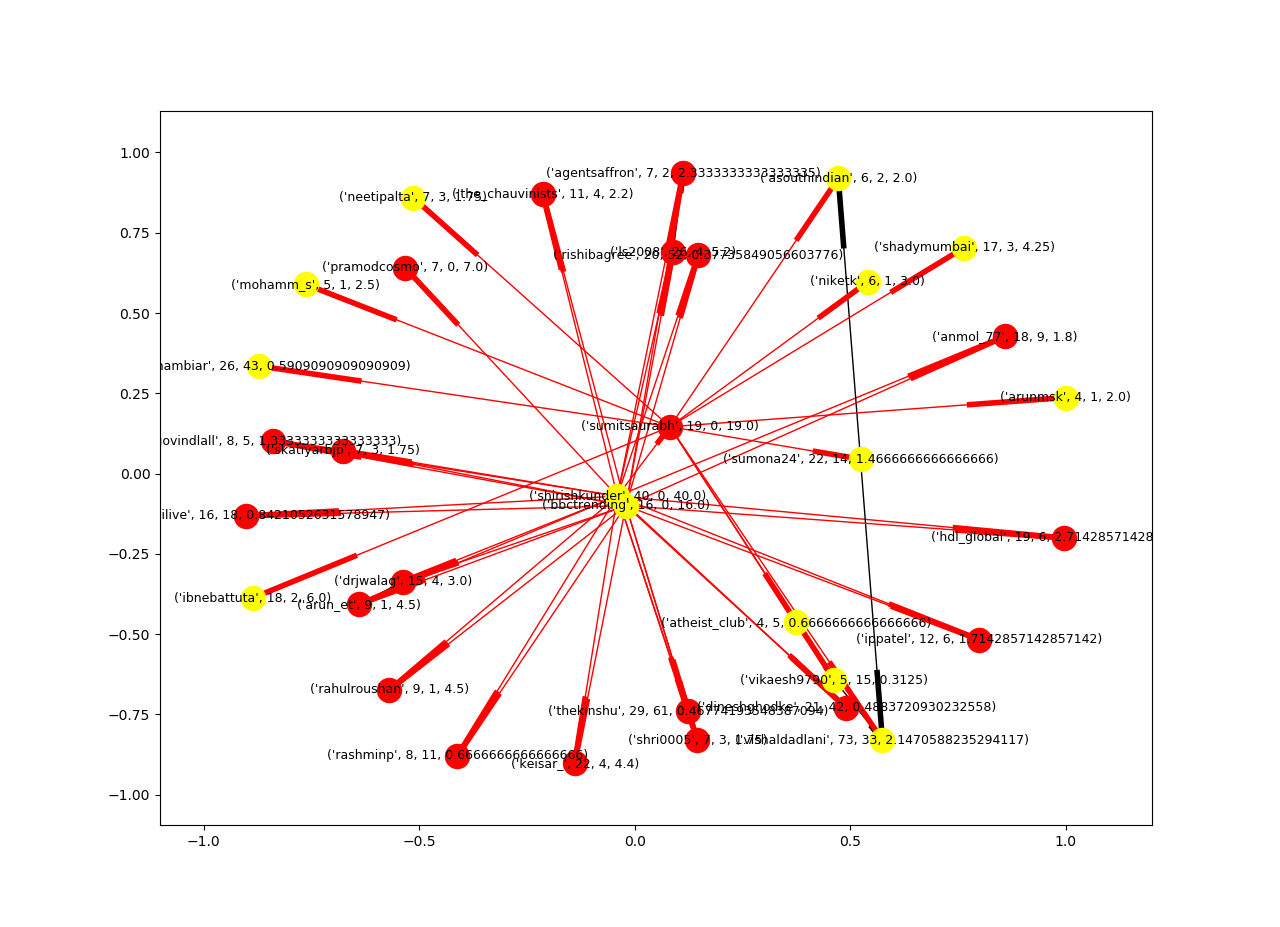
\includegraphics[scale=0.5]{images/beefban_in_degree_probability_free.png}
\end{center}
\caption{\textit{Output} tipico del \textit{tool} di visualizzazione.}
\label{fig:tool}
\end{figure}
I nodi \textit{gialli} appartengono ad una \textit{comunità} ed i nodi \textit{rossi} all'altra; gli archi evidenziati in \textit{rosso} sono i \textit{k} archi diretti scelti dall'algoritmo di \textit{k-edge recommendation} utilizzato. Si può notare come ad ogni nodo venga associato, nell'ordine, l'\textit{username} corrispondente, il suo \textit{in degree}, \textit{out degree} ed il rapporto $\frac{in degree}{out degree + 1}$.


